% !TEX program = xelatex
% 光遗传学与视网膜退化性疾病的视觉功能恢复 · 四材料十问综合题（27 分）
% 编译：xelatex -interaction=nonstopmode -halt-on-error 本文件（跑两遍）
\documentclass[UTF8,a4paper,11pt]{ctexart}

\usepackage{geometry}
\geometry{left=1.9cm,right=1.9cm,top=2.3cm,bottom=2.3cm}
\usepackage{graphicx}
\usepackage{amsmath,amssymb}
\usepackage{booktabs}
\usepackage{longtable}
\usepackage{array}
\usepackage{enumitem}
\usepackage{xcolor}
\usepackage{caption}
\usepackage{float}
\usepackage{titlesec}
\usepackage{fancyhdr}
\usepackage[hidelinks]{hyperref}

\graphicspath{{../命题图/}{../../Resources/Downloads/原图-光遗传学视觉恢复/}}

\definecolor{deepblue}{HTML}{1F4E79}
\definecolor{deepred}{HTML}{C00000}
\definecolor{deepgreen}{HTML}{2E7D32}

\captionsetup{font=small,labelfont=bf}
\titleformat{\section}{\Large\bfseries\color{deepblue}}{\thesection}{0.6em}{}
\titleformat{\subsection}{\normalsize\bfseries\color{deepblue}}{\thesubsection}{0.6em}{}
\pagestyle{fancy}
\fancyhf{}
\fancyhead[L]{\small 光遗传学与视觉功能恢复 · 四材料十问（27 分）}
\fancyhead[R]{\small\thepage}

\newcommand{\pt}[1]{\textbf{（#1分）}}
\newcommand{\lv}[1]{{\small\color{deepgreen}［#1］}}
\newcommand{\key}[1]{\textbf{\color{deepred}#1}}
\newcommand{\tian}[1]{\underline{\hspace{#1}}}
\newcommand{\choice}[1]{\par\smallskip\noindent #1\par}

\title{\bfseries 光遗传学与视网膜退化性疾病的视觉功能恢复\\[5pt]
\large 四材料 · 十问综合题（27 分）}
\author{}\date{2026-10-06}

\begin{document}
\maketitle
\thispagestyle{fancy}

\begin{center}
\fbox{\parbox{0.95\textwidth}{\small
\textbf{阅读提示}：本题所有科研事实取自 Pan et al. 2014、Lu et al. 2016、Lu et al. 2018 三篇开放获取论文。
题目中出现的专业名词，均在材料或图表注释中\textbf{给出了做题所需的全部解释}，不需要事先记忆。
凡标"\key{命题简化}"的数据，其\emph{量级与具体数值}为命题需要而设定，\emph{变化趋势}依原论文结果改写。
}}
\end{center}

\section*{命题说明}
\addcontentsline{toc}{section}{命题说明}

\noindent\textbf{核心科学问题}：如何通过"光敏蛋白性质优化 + 目标细胞靶向表达 + 功能性评价"，获得更有效的视觉恢复方案。

\begin{table}[H]
\centering\small
\begin{tabular}{@{}clp{5.6cm}cc@{}}
\toprule
\textbf{题号} & \textbf{对应材料} & \textbf{考查落点} & \textbf{难度} & \textbf{分值} \\
\midrule
Q1 & 材料一 & 视网膜细胞分工与视觉信号通路 & 基础 & 3 \\
Q2 & 材料一 & 基因表达 → 蛋白质功能 → 细胞功能 & 中等 & 3 \\
Q3 & 材料二 & 读表比较（光敏性） & 基础 & 2 \\
Q4 & 材料二 & 多指标权衡，优势与局限 & 拔高 & 3 \\
Q5 & 材料三 & 据表判断方案，细胞特异性表达 & 中等 & 3 \\
Q6 & 材料三 & 表达量 ≠ 功能（证据层级） & 拔高 & 3 \\
Q7 & 材料四 & 双因素读表比较 & 中等 & 2 \\
Q8 & 材料四 & 实验变量分析 & 中等 & 3 \\
Q9 & 材料四 & 对照的作用与评价指标的选择 & 拔高 & 2 \\
Q10 & 综合 & 开放优化方案与依据 & 拔高 & 3 \\
\midrule
\multicolumn{4}{r}{\textbf{合计}} & \textbf{27} \\
\bottomrule
\end{tabular}
\end{table}

\noindent\textbf{题型分布}：单选 1（Q7-1）、编号排序/填空 1（Q3）、编号选填 1（Q5-1）、表格与数据填空 2（Q7-2、Q8）、简答与分析 5（Q1、Q2、Q4、Q6、Q9）、开放综合 1（Q10）——以简答为主、客观题为辅，符合等级考"情境化设问 + 分层能力考查"的取向。

\section{材料一\quad 视觉损伤与治疗思路}
\addcontentsline{toc}{section}{材料一：视觉损伤与治疗思路}

视网膜像一台"光信号转换器"，把进入眼内的光变成神经信号送往大脑。视网膜中的\textbf{感光细胞}（视杆细胞与视锥细胞）负责\textbf{感受光并把光信号转变为电信号}；信号随后经\textbf{双极细胞}传到\textbf{神经节细胞}，后者的轴突汇聚成视神经，把信号送往大脑皮层视觉中枢，最终形成视觉（图1）。

视网膜色素变性（RP）是一类由基因突变引起的遗传性眼病。患者的\textbf{感光细胞逐渐死亡}，而内层的双极细胞与神经节细胞大多仍然存活。由于信号的"第一站"缺失，患者即使眼球结构和视神经通路完好，视觉功能仍会逐渐下降（图1）。

研究者尝试用\textbf{光遗传学}方法恢复视觉：把一种来自单细胞藻类的\textbf{光敏蛋白基因（ChR2 基因）}导入残存的视网膜细胞。ChR2 蛋白的特点是：它能在细胞膜上形成\textbf{受光控制的离子通道}——受到蓝光照射时通道开放，阳离子内流，细胞因此产生电位变化。

\begin{figure}[H]
\centering
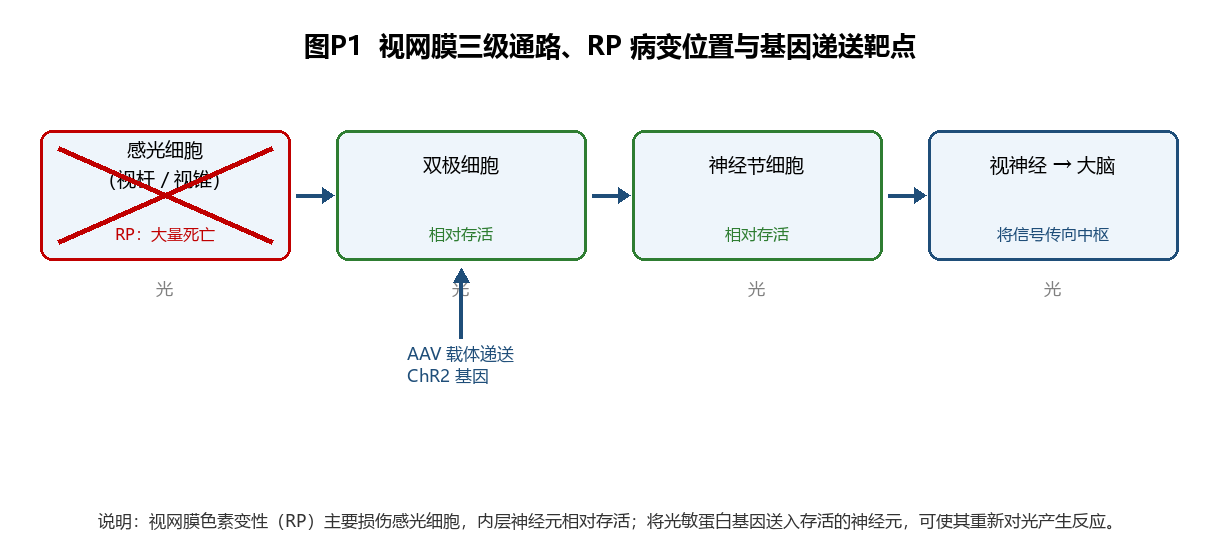
\includegraphics[width=0.95\textwidth]{P1_视网膜三级通路与病变.png}
\caption{图1\quad 视网膜三级细胞通路、RP 的主要受损环节与治疗靶点（简化示意图）}
\end{figure}

\subsection*{问题}

\begin{enumerate}[leftmargin=2.2em,itemsep=5pt]
\item \lv{基础} \pt{3} 根据图1 与材料信息，分析感光细胞退化为什么会引起视觉功能下降。

\item \lv{中等} \pt{3} 研究者把 ChR2 基因导入残存的视网膜神经细胞后，这些细胞便能在蓝光照射下产生反应。结合材料，说明这一过程发生的可能机制（要求体现"基因表达 → 蛋白质功能 → 细胞功能"的链条）。
\end{enumerate}

\section{材料二\quad ChR2 突变体}
\addcontentsline{toc}{section}{材料二：ChR2 突变体}

天然 ChR2 有一个明显不足：需要在较强的光下才能被有效激活。研究者通过改变 ChR2 基因中特定位置的碱基序列，获得了多种\textbf{突变体}，并测定了它们的性能（表1）。

\begin{table}[H]
\centering\small
\caption*{\textbf{表1}\quad ChR2 及其突变体的性能比较（\key{命题简化}数据，相对值）}
\begin{tabular}{@{}lcccc@{}}
\toprule
\textbf{变体} & \textbf{阈值光强} & \textbf{弱光下光电流} & \textbf{通道关闭时间（响应时间）} & \textbf{高频闪烁下的响应能力} \\
\midrule
wt-ChR2（天然型） & 10 & 1.0 & 最短 & 强 \\
ChR2-L132C & 4 & 2.4 & 较长 & 中 \\
ChR2-L132C/T159C & 3 & 3.1 & 长 & 弱 \\
ChR2-L132C/T159S & 2 & 4.0 & 最长 & 很弱 \\
\bottomrule
\end{tabular}

\smallskip
\parbox{0.94\textwidth}{\footnotesize 注：\textbf{阈值光强}指能使细胞产生可检测光电流所需的最低光强，数值越小表示在越弱的光下即可被激活；\textbf{光电流}是通道开放时通过的离子流形成的电流，光电流越大表示对光越敏感；\textbf{通道关闭时间}指光照停止后通道关闭、细胞恢复静息状态所需的时间，时间越长表示细胞"恢复"越慢，对随时间快速变化的光信号（如闪烁、运动）的跟随能力越弱。数据为命题简化，趋势依据 Pan et al., 2014 改写。}
\end{table}

\subsection*{问题}

\begin{enumerate}[leftmargin=2.2em,itemsep=5pt,start=3]
\item \lv{基础} \pt{2} 根据表1，把四种变体按\textbf{光敏性由高到低}排序（填变体名称）：\\
\tian{2.6cm} $>$ \tian{2.6cm} $>$ \tian{2.6cm} $>$ \tian{2.6cm}

\item \lv{拔高} \pt{3} 某突变体的光敏性显著提高，但其时间响应特性有所下降。请结合表1，分析该突变体用于视觉恢复时的\textbf{优势}与\textbf{局限}，并说明这是否意味着"光敏性最高就等于视觉恢复效果最好"。
\end{enumerate}

\section{材料三\quad AAV 递送与目标细胞靶向表达}
\addcontentsline{toc}{section}{材料三：AAV 递送与靶向表达}

把基因送入细胞需要"载体"。研究者使用\textbf{腺相关病毒（AAV）}作为载体：它能把携带的基因送入细胞，且本身引起的免疫反应较弱。但仅有载体还不够——基因在\textbf{哪些细胞}里表达、表达\textbf{多少}，取决于与目的基因连接在一起的\textbf{调控元件}（启动子与增强子）：启动子决定基因在什么条件下"开启"，增强子能加强这种表达。

研究者设计了三种构建方案（方案中目的基因与载体其余部分相同，只有调控元件不同），并在小鼠视网膜中检测表达情况（表2）。图2 是把 ChR2 与红色荧光蛋白 mCherry 融合后，与能特异标记双极细胞的 PKC 抗体共同标记的结果：若红色荧光（表示基因表达）与绿色荧光（表示双极细胞）大量重叠，说明目的基因主要表达在双极细胞中。

\begin{table}[H]
\centering\small
\caption*{\textbf{表2}\quad 三种构建方案的表达情况比较（\key{命题简化}数据，相对水平）}
\begin{tabular}{@{}llccc@{}}
\toprule
\textbf{方案} & \textbf{调控元件} & \textbf{ChR2 总表达量} & \textbf{双极细胞中表达比例} & \textbf{非目标细胞中表达情况} \\
\midrule
甲 & 200 bp 增强子 + SV40 启动子 & 中 & 中 & 较明显 \\
乙 & 内源 mGluR6 启动子 + 200 bp 增强子 & 较高 & 高 & 很少 \\
丙 & 内源 mGluR6 启动子 + 内含子增强子 & 高 & 很高 & 极少 \\
\bottomrule
\end{tabular}

\smallskip
\parbox{0.94\textwidth}{\footnotesize 注：\textbf{mGluR6 调控元件}是与双极细胞中某基因表达相关的调控序列，本研究用它来提高目的基因在双极细胞中的表达；数据为命题简化，趋势依据 Lu et al., 2016 结果改写。}
\end{table}

\begin{figure}[H]
\centering
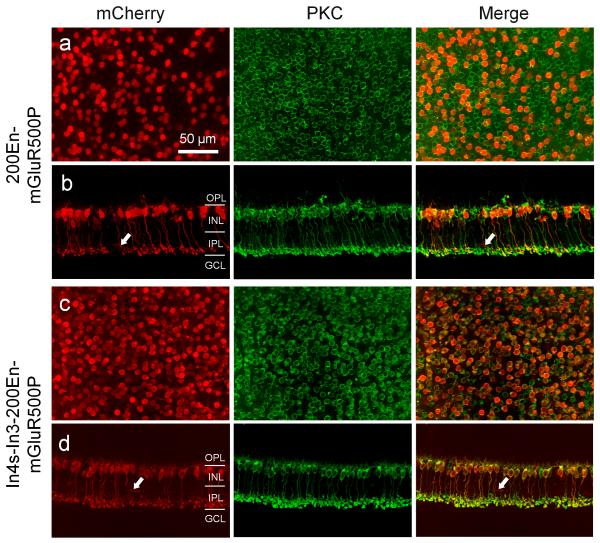
\includegraphics[width=1.0\textwidth]{Lu2016-Fig04.jpg}
\caption{图2\quad 论文原图（Lu et al., \textit{Gene Therapy}, 2016, Fig.~4）：目的基因的表达产物（红）与双极细胞标记物（绿）的共标结果}
\end{figure}

\subsection*{问题}

\begin{enumerate}[leftmargin=2.2em,itemsep=5pt,start=5]
\item \lv{中等} \pt{3}
\begin{enumerate}[label=(\arabic*),leftmargin=1.4em,itemsep=2pt]
\item 根据表2，更适合实现"目的基因主要在双极细胞中表达"的方案是\tian{0.9cm}（填"甲""乙"或"丙"）（1 分）
\item 说明你作出上述判断的理由（2 分）。
\end{enumerate}

\item \lv{拔高} \pt{3} 有同学认为："只要让视网膜细胞表达出尽可能多的 ChR2，视觉恢复效果就一定最好。"请结合材料二、材料三说明这一观点为什么不全面。
\end{enumerate}

\section{材料四\quad 用 OMR 评价视觉功能是否恢复}
\addcontentsline{toc}{section}{材料四：用 OMR 评价视觉功能是否恢复}

细胞是否"对光有反应"，不等于动物是否"看得见"。为评价视觉功能是否真正恢复，研究者使用\textbf{视动反应（OMR）}：把小鼠放在能显示移动条纹的装置中，若小鼠能看清条纹，其头部会随条纹运动方向转动；条纹越密集（\textbf{空间频率}越高），看清越困难，需要的光也越强。

研究者把三种 ChR2 变体分别导入三组同种失明小鼠，并设置一组\textbf{未经相同基因治疗处理}的小鼠作对照，测定了各组出现 OMR 所需的最低光强（表3）。

\begin{table}[H]
\centering\small
\caption*{\textbf{表3}\quad 各组小鼠出现 OMR 所需的最低光强（\key{命题简化}数据，相对值；"—"表示未出现 OMR）}
\begin{tabular}{@{}lccc@{}}
\toprule
\textbf{组别} & \textbf{低空间频率} & \textbf{中空间频率} & \textbf{高空间频率} \\
\midrule
未经基因治疗的对照组 & — & — & — \\
wt-ChR2 组 & 20 & $>$40 & — \\
ChR2-L132C 组 & 12 & 22 & $>$50 \\
ChR2-L132C/T159C 组 & 8 & 15 & 30 \\
ChR2-L132C/T159S 组 & 5 & 9 & 18 \\
\bottomrule
\end{tabular}
\end{table}

\subsection*{问题}

\begin{enumerate}[leftmargin=2.2em,itemsep=5pt,start=7]
\item \lv{中等} \pt{2}
\begin{enumerate}[label=(\arabic*),leftmargin=1.4em,itemsep=2pt]
\item 在相同条件下，视觉功能恢复效果最好的一组是\tian{3.6cm}（填变体名称）（1 分）
\item 根据表3，随空间频率升高，各组出现 OMR 所需的最低光强均\tian{1.2cm}，这说明\tian{0.42\textwidth}（1 分）
\end{enumerate}

\item \lv{中等} \pt{3} 若研究目的是"比较两种 ChR2 突变体对视觉恢复的影响"，请写出该实验的\textbf{自变量}、\textbf{因变量}，以及至少两个需要控制相同的变量。\tian{0.5\textwidth}

\item \lv{拔高} \pt{2} 请回答下列两个问题：
\begin{enumerate}[label=(\arabic*),leftmargin=1.4em,itemsep=2pt]
\item 为什么必须设置"未经相同基因治疗处理"的对照组？（1 分）
\item 为什么不能仅通过检测视网膜中 ChR2 的\textbf{表达量}来评价治疗效果？（1 分）
\end{enumerate}
\end{enumerate}

\section{综合题}
\addcontentsline{toc}{section}{综合题}

\begin{enumerate}[leftmargin=2.2em,itemsep=5pt,start=10]
\item \lv{拔高·开放} \pt{3} 研究者希望进一步优化治疗方案。请根据上述全部材料，从"\textbf{ChR2 本身}、\textbf{目标细胞表达}、\textbf{刺激条件}、\textbf{功能评价}"中选择一个或多个角度，提出一种合理的优化思路，并说明依据。
\end{enumerate}

\clearpage
\section*{参考答案与评分细则}
\addcontentsline{toc}{section}{参考答案与评分细则}

\begin{longtable}{@{}p{0.9cm}p{9.6cm}p{4.2cm}@{}}
\toprule
\textbf{题} & \textbf{参考答案} & \textbf{评分点} \\
\midrule
\endhead
Q1 & 感光细胞的功能是感受光并把光信号转变为电信号，是视网膜形成视觉信号的\textbf{第一站}；感光细胞退化死亡后，光信号无法在这里转变为神经信号，位于其下游的双极细胞、神经节细胞虽然存活却\textbf{得不到输入}，视网膜无法向大脑输出信号，因此视觉功能下降（严重时失明）。 & 说出感光细胞的功能（光信号→电信号）1 分；指出信号在视网膜第一站中断 1 分；体现"下游细胞存活但无输入"1 分。仅答"因为细胞死了"不得分。 \\
\addlinespace
Q2 & 导入的 ChR2 基因在细胞内\textbf{转录、翻译}出 ChR2 蛋白；该蛋白\textbf{定位到细胞膜上}，形成能被光控制的离子通道；蓝光照射时通道开放、阳离子内流，使\textbf{膜电位发生改变}，细胞由此产生电信号（光响应）。 & 基因表达出蛋白 1 分；蛋白定位于膜上并形成受光调控的通道 1 分；光照→离子内流→膜电位改变→产生电信号 1 分。缺少"膜电位改变/产生电信号"扣 1 分。 \\
\addlinespace
Q3 & ChR2-L132C/T159S $>$ ChR2-L132C/T159C $>$ ChR2-L132C $>$ wt-ChR2 & 顺序完全正确得 2 分；顺序错误或漏项得 0 分。 \\
\addlinespace
Q4 & \textbf{优势}：该突变体阈值光强最低、弱光下光电流最大，即在很弱的光下即可被激活，适合在弱光环境（如夜间、室内）中产生光响应。\textbf{局限}：其通道关闭时间最长，细胞恢复静息慢，对随时间快速变化的光信号（高频闪烁、运动）的跟随能力最差，可能导致动态视觉信息难以分辨。\textbf{结论}：光敏性高只是"更容易被激活"，而视觉恢复还要求能分辨随时间变化的信息，故"光敏性最高"不等于"恢复效果最好"。 & 优势（弱光下易被激活）1 分；局限（响应变慢→动态分辨下降）1 分；得出"需在多指标间权衡、光敏性最高≠恢复最好"1 分。只答"它更敏感"不得分。 \\
\addlinespace
Q5 & (1) \textbf{丙}。(2) 丙方案在目标细胞（双极细胞）中的表达比例最高、在非目标细胞中的表达极少，说明其调控元件能使目的基因\textbf{主要在双极细胞中表达}，细胞特异性最好；同时其总表达量也最高，为产生足够的光响应提供了基础。 & (1) 填"丙"1 分。(2) 依据"目标细胞比例高"1 分；依据"非目标细胞表达少（特异性）"或"总表达量高（为功能提供基础）"1 分。只答"丙最好"未给理由不得分。 \\
\addlinespace
Q6 & 不全面。① 表达量只说明细胞里产生了多少 ChR2 蛋白，属于\textbf{蛋白水平}，是必要条件而非充分条件；② 材料三表明，若表达发生在\textbf{非目标细胞}中，既不能形成有效的视觉信号，还可能干扰视网膜原有的信号处理；③ 材料二表明，蛋白\textbf{功能是否合适}还取决于响应时间等指标——光敏性高但响应慢不利于分辨动态信息；④ 最终还必须看动物\textbf{行为水平}上（OMR）是否真正出现功能改善。 & 指出"表达量是蛋白水平、必要但不充分"1 分；答出"须表达在正确的细胞"或"蛋白功能（响应时间）要合适"1 分；答出"需以行为学等功能性指标为准"1 分。 \\
\addlinespace
Q7 & (1) \textbf{ChR2-L132C/T159S 组}。(2) 随空间频率升高，各组所需的最低光强均\key{升高}；这说明条纹越密集越难分辨，需要更强的光才能引出 OMR（即空间频率升高会降低视觉分辨的灵敏度）。 & (1) 1 分。(2) 填"升高"0.5 分，解释合理 0.5 分。 \\
\addlinespace
Q8 & \textbf{自变量}：导入的 ChR2 突变体类型（并设未经相同基因治疗处理的对照组）。\textbf{因变量}：是否出现 OMR、出现 OMR 所需的最低光强（阈值光强）。\textbf{控制变量}（答出两个）：小鼠的遗传背景与生理状态（同一失明模型）、注射的载体量与浓度、注射后至测定的时间、光刺激的波长与强度、条纹的空间频率等。 & 自变量 1 分（须体现"不同突变体"且含对照）；因变量 1 分；控制变量答出两个 1 分。 \\
\addlinespace
Q9 & (1) 设置未经相同基因治疗处理的对照组，是为了排除"失明小鼠本身、注射操作或光刺激"等因素也能引起 OMR 的可能，从而证明观察到的反应\textbf{确实来自导入的 ChR2}，使因果判断成立。(2) ChR2 表达量只反映蛋白的多少，而治疗效果是动物\textbf{整体视觉功能}的表现；表3 显示各组都能表达 ChR2，但出现 OMR 所需的最低光强明显不同，说明表达量相近时功能表现仍可不同，因此应以\textbf{行为学等功能性指标}评价疗效。 & 对照的作用（排除其他因素、证明因果）1 分；表达量≠功能、须用功能性指标 1 分。 \\
\addlinespace
Q10 & 角度与依据（答出一个角度并说明依据即可）：\textbf{① ChR2 本身}——在保持较高光敏性的同时筛选响应更快的变体（依据 Q4/Q7：光敏性与响应时间存在权衡，响应快有利于分辨运动信息）。\textbf{② 目标细胞表达}——进一步优化调控元件，使表达更集中于双极细胞（依据 Q5/Q6：非目标细胞表达少可减少干扰、提高特异性）。\textbf{③ 刺激条件}——优化光刺激的波长、强度与频率，使之与所用变体匹配（依据 Q4/Q7：不同变体对不同光强、不同模式刺激的响应不同）。\textbf{④ 功能评价}——增加瞳孔对光反射、多空间频率下的 OMR 等指标，避免以单一指标判断疗效（依据 Q7/Q9：功能评价应多层次）。 & 优化方向合理且能从前文推出 1 分；依据与方向匹配并引用具体材料或数据 1 分；表述完整、逻辑清楚 1 分。方向脱离材料（如"用干细胞替换视网膜"）不得分。 \\
\bottomrule
\end{longtable}

\noindent\textbf{难度分层}：基础 5 分（Q1、Q3）；中等 11 分（Q2、Q5、Q7、Q8）；拔高 11 分（Q4、Q6、Q9、Q10）。\textbf{主要区分点}：Q4（多指标权衡）、Q6（表达量≠功能）、Q10（证据整合下的开放设计）。

\clearpage
\section*{命题底线自检}
\addcontentsline{toc}{section}{命题底线自检}

\begin{longtable}{@{}p{0.6cm}p{6.2cm}p{8.0cm}@{}}
\toprule
\textbf{\#} & \textbf{底线要求} & \textbf{落实情况} \\
\midrule
\endhead
1 & 不要求学生背诵 ChR2、mGluR6、AAV 的专业定义 & 三者均以"材料给定的含义"出现：ChR2 是"受蓝光控制开闭的离子通道蛋白"，AAV 是"能把基因送入细胞的载体"，mGluR6 调控元件是"与双极细胞表达相关的调控序列"。答案中无一处要求定义式记忆。 \\
\addlinespace
2 & 材料中首次出现的专业事实必须给出必要解释 & 阈值光强、光电流、通道关闭时间、高频闪烁响应、空间频率、OMR、启动子/增强子、共标（重叠）均在材料或表注中解释。 \\
\addlinespace
3 & 不使用大学电生理学作为直接考点 & 全题未要求解释动作电位的离子机制、通道动力学方程或膜片钳原理；"响应时间"只作为表中给定信息用于比较。 \\
\addlinespace
4 & 不要求学生记忆论文中的实验编号、载体编号、品系名称 & 未出现任何载体编号、血清型、小鼠品系名称；仅保留"失明小鼠""对照组"这类功能性表述。 \\
\addlinespace
5 & 专业数据应经过高中化处理 & 表1—表3 均为相对值并标注"命题简化"，趋势依原文改写；未直接搬运论文原始数值或图注编号。 \\
\addlinespace
6 & 高难度来自多证据整合，而非术语陌生度 & Q4（表1 两列指标权衡）、Q6（材料二＋材料三整合）、Q10（四段材料整合）的难点都在证据整合与变量分析；术语本身不构成难点。 \\
\addlinespace
7 & 每一个结论都必须有材料或高中知识支持 & 逐问核查：Q1（图1＋教材概念）、Q2（材料一给定 ChR2 作用方式）、Q3/Q4（表1）、Q5（表2）、Q6（表1＋表2）、Q7/Q8/Q9（表3）、Q10（前文全部）。无一处需要材料外的信息。 \\
\bottomrule
\end{longtable}

\section*{附录\quad 论文原图对照（课堂延伸用）}
\addcontentsline{toc}{section}{附录：论文原图对照}

\begin{figure}[H]
\centering
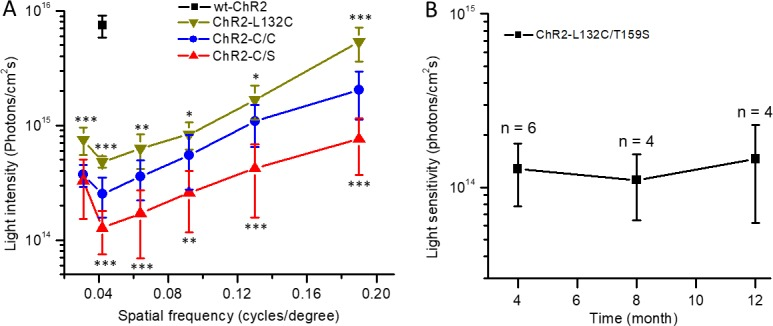
\includegraphics[width=1.0\textwidth]{Lu2018-Fig04.jpg}
\caption{图A\quad 论文原图（Lu et al., \textit{IOVS}, 2018, Fig.~4）：三种 ChR2 变体的 OMR 阈值光强—空间频率关系，与表3 的趋势一致，供课堂延伸或更换命题数据时对照使用。}
\end{figure}

\noindent\small 全部 22 张论文原图与三篇文献（两篇全文 Markdown、一篇原版 PDF）存于 \texttt{00 - Personal/Resources/Downloads/}。

\end{document}
